\chapter{Game Theory}\label{ch:gametheory}

\section{Games}\label{sec:games}

Game theory studies situations in which an agent faces one or more
choices whose combined outcome depends on the choices of other agents.
Such situations are called \textbf{games}, and the agents
\textbf{players}. The Prisoner's Dilemma (example \ref{ex:pd}) is a game
in this sense, because the outcome of your choice (confessing or
remaining silent) depends on what your partner decides to do.

Whenever an agent faces a choice in a game, the MEU Principle tells us
that she ought to choose whichever option maximizes expected
utility. We don't need a new decision theory for
games. Nonetheless, there are reasons for studying the special case
where the states in a decision problem are other people's (real or
potential) actions.

One reason is that game theory can shed light on important political
and social issues. The Prisoner's Dilemma, for instance, illustrates a
common type of situation in which everyone pursuing their own interest
leads to a worse result for everyone than what could otherwise have been
achieved. Any such situation is nowadays called a Prisoner's Dilemma,
even if no prisoners are involved. For example, if you're a
professional athlete, you have an incentive to use steroids, no matter
whether your competitors do the same. Without strict controls, the
outcome is that everyone uses steroids, even though everyone would
prefer that no-one uses steroids. The athletes face a Prisoner's
Dilemma. For another example, if you're a fisherman, you have an
incentive to catch as many fish as you can, even though everyone would
be better off if everyone restrained themselves to sustainable quotas.

Thomas Hobbes (in effect) argued that the pervasiveness of Prisoner's
Dilemmas justifies the subordination of people under a state. It is in
everyone's interest to impose a system of control and punishment that
ensures the best outcome in what would otherwise be a Prisoner's
Dilemma.

\cmnt{%
  The only way to make rational agents not be trapped in the PD is to
  change the payoffs. This could result in a variety of
  ways. Contracts, enforcement, morality, etc.
} %

Another reason to study games is that a new set of conceptual tools
and techniques become available if the outcomes depend on other
people's choices. For example, game theorists typically don't specify the
probability of the states -- that is, of the other players'
actions. Instead, they specify the utility of the outcomes for all
players. Under certain assumptions, this is enough to figure out what
each player will do.

Here is how game theorists would write the matrix
for the original Prisoner's Dilemma, assuming you and your partner only
care about your own prison terms:
\begin{center}
  \begin{tabular}{|r|c|c|}\hline
    \gr & \gr Confess & \gr Silent\\\hline
    \gr Confess & -5,-5 & 0,-8  \\\hline
    \gr Silent & -8,0 & -1,-1 \\\hline
  \end{tabular}
\end{center}
The rows are the acts available to you, as before; the columns are the
acts available to your partner. The numbers in the cells represent the
utility of the relevant outcome for you and your partner. We usually
don't describe the outcome itself anymore (for lack of space). In a
two-player matrix, the first number in each cell is always the utility
for the row player (whom we'll call `Row'); the second is the utility
for the column player (`Column').

% \begin{exercise1}
%   Draw the game matrix for the Prisoner Dilemma, assuming you
%   only care about your own prison term, but your partner cares equally
%   about both of you.
% \end{exercise1}

In the above matrix, it is clear that each player will confess,
because confessing dominates remaining silent: it is better no matter
what the other player does.

Now consider the following matrix, for a different kind of game. 
\begin{center}
  \begin{tabular}{|r|c|c|}\hline
    \gr & \gr $C_1$ & \gr $C_2$ \\\hline
    \gr $R_1$ & 2,2 & 1,3 \\\hline
    \gr $R_2$ & 1,1 & 2,2 \\\hline
  \end{tabular}
\end{center}
Row no longer has a dominant option. What she should do depends on
what she thinks Column will do. If Column chooses $C_1$, then Row
should play $R_1$; if Column chooses $C_2$, then Row should play
$R_2$. Can we nonetheless say what Row will do without specifying her
beliefs? 

Look at the game from Column's perspective. No matter what Row does,
Column is better off choosing $C_2$. In other words, $C_2$ dominates
$C_1$. So if Row knows the utility Column assigns to the outcomes, she
can figure out that Column will choose $C_2$. And so Row should choose
$R_2$. The ``solution'' of the game is therefore the pair of options
$(R_2,C_2)$ -- meaning that if Column and Row are rational players
knowing about each other's utilities, then Row will choose $R_2$ and
Column $C_2$.

Here is another, more complex example.
\begin{center}
  \begin{tabular}{|r|c|c|c|}\hline
    \gr & \gr $C_1$ & \gr $C_2$ & \gr $C_3$ \\\hline
    \gr $R_1$ & 0,1 & 2,2 & 3,1 \\\hline
    \gr $R_2$ & 2,2 & 1,3 & 2,2 \\\hline
    \gr $R_3$ & 1,1 & 0,2 & 0,3 \\\hline
  \end{tabular}
\end{center}
From Row's perspective, $R_1$ is the best choice if Column plays $C_2$
or $C_3$, and $R_2$ is the best choice if Column goes for $C_1$. For
Column, $C_2$ is the best choice in case of $R_1$ or $R_2$, and $C_3$
is best in case of $R_3$. But Column can hardly expect Row to choose
$R_3$, since $R_3$ is dominated by $R_2$. So Column can figure out
that Row will play either $R_1$ or $R_2$, which means that Column will
play $C_2$. And since Row can figure out that Column will play $C_2$,
Row will play $R_1$. The solution is $(R_1,C_2)$.

\cmnt{%
  The reason why Row won't choose $R_3$ is that it is strictly
  dominated by both $R_1$ and $R_2$. In general, option $A$ is
  strictly dominates option $B$ if its outcome is better in every
  state. We say that an option is \emph{dominated} if there is some
  other option that dominates it. In the example, $R_3$ is
  dominated. Notice that it is not enough for $A$ to be dominated that
  in every state, some option or other is better than $A$. There has
  to be a single option that is better in every state.
} %

\cmnt{%
  The procedure by which we solved the previous game is called
  \emph{iterative deletion of dominated strategies}. The idea is that
  we always delete dominated options until only one cell is left.
} %

Note that to reach this conclusion it is not enough to assume that
both players know each other's utilities. For one thing, the players
must also know that none of them will choose a dominated
act. Moreover, to figure out that Column will play $C_2$, Row needs
to know that Column knows her (Row's) utilities, and she needs to know
that Column knows that she (Row) won't choose a dominated option.

In general, game theorists usually assume that
\begin{enumerate*}
\itemsep0em
\item[(1)] all players know the options and utilities of all other players;
\item[(2)] all players know that all other players are rational;
\item[(3)] all players know that (1)--(3) are satisfied.
\end{enumerate*}
By applying to itself, the last clause ensures that (1) and (2) hold
with arbitrarily many iterations of `all players know that' stacked in
front. If something is in this way known by everyone, and known by
everyone to be known by everyone, and so on, then it is said to be
\textbf{common knowledge}. So (1)--(3) say that the options and
utilities of all players, as well as all players' rationality, are
common knowledge. This is obviously an idealization. We'll see below
that it gives rise to some interesting puzzles.

\begin{exercise2}\label{e:elim-dom-strat}
  Under the assumptions (1)--(3), what will Row and Column do in the following games?
  \begin{center}
    \begin{tabular}{lll}
      a. \begin{tabular}[t]{|r|c|c|c|}
        \gr & \gr $C_1$ & \gr $C_2$ \\\hline
        \gr $R_1$ & 1,0 & 1,2  \\\hline
        \gr $R_2$ & 0,3 & 0,1 \\\hline
      \end{tabular}&
      b. \begin{tabular}[t]{|r|c|c|c|}
        \gr & \gr $C_1$ & \gr $C_2$ & \gr $C_3$ \\\hline
        \gr $R_1$ & 1,0 & 1,2 & 0,1 \\\hline
        \gr $R_2$ & 0,3 & 0,1 & 2,0 \\\hline
      \end{tabular}&
      \cmnt{%
        $C_3$ is dominated by $C_2$; having removed $C_3$, $R_2$ is dominated by $R_1$.
      } %
      c. \begin{tabular}[t]{|r|c|c|c|}
        \gr & \gr $C_1$ & \gr $C_2$ & \gr $C_3$ \\\hline
        \gr $R_1$ & 0,1 & 2,0 & 2,4 \\\hline
        \gr $R_2$ & 4,3 & 1,4 & 2,5 \\\hline
        \gr $R_3$ & 2,4 & 3,6 & 3,1 \\\hline
      \end{tabular}
      \cmnt{%
        $R_1$ is dominated by $R_3$; then $C_1$ by $C_2$; then $R_2$ by $R_3$. So R2,C3.
      } %
    \end{tabular}
  \end{center}
\end{exercise2}

\section{Nash equilibria}

Have a look at this game.
\begin{center}
  \begin{tabular}{|r|c|c|c|}\hline
    \gr & \gr $C_1$ & \gr $C_2$ & \gr $C_3$ \\\hline
    \gr $R_1$ & 4,2 & 2,3 & 3,1 \\\hline
    \gr $R_2$ & 3,1 & 3,2 & 4,1 \\\hline
    \gr $R_3$ & 4,2 & 1,1 & 0,3 \\\hline
  \end{tabular}
\end{center}
No option for either player is dominated by any other. Nonetheless,
game theory says that we can figure out what each player will choose. 

Let's start with some trial and error. Take $(R_1,C_1)$. Could this be
the outcome that is reached whenever the game is played by two players
under the idealizing assumptions (1)--(3)? No. Otherwise Column
would know that Row is going to play $R_1$. And then Column is better
off playing $C_2$. The opposite happens with $(R_1,C_2)$: if Row knew
that Column plays $C_2$, she would be better off playing $R_2$. The
same reasoning disqualifies all other combinations except $(R_2,C_2)$ --
the middle cell. If Row knows that Column is going to play $C_2$, she
can do no better than play $R_2$. Likewise for Column: if Column knows
that Row is going to play $R_2$, she can do no better than play $C_2$.

A combination of options that is ``stable'' in this way is called a
\textbf{Nash equilibrium} (after the economist John Nash). In general,
a Nash equilibrium is a combination of acts, one for each player, such
that no player could get greater utility by deviating from her part of
the equilibrium given that the other players stick to their part.

Here is an algorithm for finding Nash equilibria. Start from the
perspective of the row player. For each act of the column player,
underline the best outcome(s) Row can achieve if Column chooses this
act. In the example above, you would underline the 4s in the first
column, the 3 in the middle cell, and the 4 in the third column. Then
do the same with the column player: for each act of Row, underline the
best possible outcome(s) for Column. The result looks like this.
\begin{center}
  \begin{tabular}{|r|c|c|c|}\hline
    \gr & \gr $C_1$ & \gr $C_2$ & \gr $C_3$ \\\hline
    \gr $R_1$ & \underline{4},2 & 2,\underline{3} & 3,1 \\\hline
    \gr $R_2$ & 3,1 & \underline{3},\underline{2} & \underline{4},1 \\\hline
    \gr $R_3$ & \underline{4},2 & 1,1 & 0,\underline{3} \\\hline
  \end{tabular}
\end{center}
Any cell in which both numbers are underlined identifies a Nash
equilibrium.

According to standard game theory, if a game has a unique Nash
equilibrium, and assumptions (1)--(3) hold, then the players will play
their part of the equilibrium. 

This is not as obvious as it may perhaps appear. Consider the next
game.
\begin{center}
  \begin{tabular}{|r|c|c|c|}\hline
    \gr & \gr $C_1$ & \gr $C_2$ & \gr $C_3$ \\\hline
    \gr $R_1$ & \underline{2},-2 & -1,\underline{1} & \underline{1},-1 \\\hline
    \gr $R_2$ & 0,0 & \underline{0},0 & -2,\underline{2} \\\hline
    \gr $R_3$ & 0,\underline{0} & \underline{0},\underline{0} & \underline{1},-1 \\\hline
  \end{tabular}
\end{center}
Here $(R_3,C_2)$ is the unique Nash equilibrium. According to game
theory, if you're Row, you can therefore be sure that Column will play
$C_2$. But if you're sure that Column will play $C_2$, then $R_2$ and
$R_3$ have equal expected utility! So it is not obvious that you have
to play $R_3$.

To be sure, if you played $R_2$ and Column could predict your choice,
then Column would play $C_3$, leaving you worse off. But we're not
assuming that Column can predict your choice. All we're assuming is
(1)--(3). Still, there is an argument in favour of
$(R_3,C_2)$. Suppose for reductio that under assumptions (1)--(3) you
could just as well play $R_2$ or $R_3$. Then Column couldn't be sure
which of these you choose; she would have to give roughly equal
credence to $R_2$ and $R_3$. But then it is best for her to choose
$C_3$. Anticipating this, you would then have to choose $R_3$. This
contradicts our assumption that you could just as well play $R_2$ or
$R_3$.



\cmnt{%

  That's strange. We have a violation of MEUP. Really, $R_2$ and $R_3$
  are both permissible but Row can't resolve to choose $R_3$ in
  deliberation?

} %


\begin{exercise1}\label{e:ne}
  Identify the Nash equilibria in the following games.
  \begin{center}
    \begin{tabular}{lll}
      a. \begin{tabular}[t]{|r|c|c|}
        \gr & \gr $C_1$ & \gr $C_2$  \\\hline
        \gr $R_1$ & 3,4 & 4,3  \\\hline
        \gr $R_2$ & 1,3 & 5,2  \\\hline
        \gr $R_3$ & 2,0 & 1,5  \\\hline
      \end{tabular} &
      b. \begin{tabular}[t]{|r|c|c|c|}
        \gr & \gr $C_1$ & \gr $C_2$ & \gr $C_3$ \\\hline
        \gr $R_1$ & 1,0 & 1,2 & 0,1 \\\hline
        \gr $R_2$ & 0,3 & 0,1 & 2,0 \\\hline
      \end{tabular}&
      \cmnt{%
        $C_3$ is dominated by $C_2$; having removed $C_3$, $R_2$ is dominated by $R_1$.
      } %
      c. \begin{tabular}[t]{|r|c|c|c|}
        \gr & \gr $C_1$ & \gr $C_2$ & \gr $C_3$ \\\hline
        \gr $R_1$ & 0,1 & 2,0 & 2,4 \\\hline
        \gr $R_2$ & 4,3 & 1,4 & 2,5 \\\hline
        \gr $R_3$ & 2,4 & 3,6 & 3,1 \\\hline
      \end{tabular}
      \cmnt{%
        $R_1$ is dominated by $R_3$; then $C_1$ by $C_2$; then $R_2$ by $R_3$. So R2,C3.
      } %
    \end{tabular}
  \end{center}
\end{exercise1}

\begin{exercise2}
  Whenever the method from section \ref{sec:games}, which is called
  \textbf{elimination of dominated strategies}, identifies a
  combination of acts as a game's solution, then that combination of
  acts is a Nash equilibrium. Can you explain why?
\end{exercise2}

\section{Zero-sum games}

In some games, the players' preferences are exactly opposed: if Row
prefers a given outcome to another by a certain amount, then Column
prefers the second outcome to the first by the same amount.  The
utilities in every cell therefore sum to the same amount. Since
utility scales don't have a fixed zero, game theorists usually
re-scale the utilities so that the sum is zero. For that reason, games
in which the agents' preferences are exactly opposed are called
\textbf{zero-sum games}. Here is an example.

\begin{center}
  \begin{tabular}{|r|c|c|c|}\hline
    \gr & \gr $C_1$ & \gr $C_2$ & \gr $C_3$ \\\hline
    \gr $R_1$ & 1,\underline{-1} & \underline{3},-3 & \underline{1},\underline{-1} \\\hline
    \gr $R_2$ & \underline{2},-2 & -2,\underline{2} & -1,1 \\\hline
  \end{tabular}
\end{center}

$(R_1,C_3)$ is the unique Nash equilibrium. It is also a combination
of the players' maximin strategies. Recall that according to the
maximin rule, you should choose whichever option has the best
worst-case outcome. In the example, the worst-case outcome of $R_1$
(for Row) is utility 1; for $R_2$ it is -2. So maximin says that Row
should choose $R_1$. Similarly, it says that Column should choose
$C_3$. And that's just our Nash Equilibrium.

In section \ref{sec:solving}, I argued that maximin is an indefensible
decision rule. But it makes sense in the context of zero-sum games,
under assumptions (1)--(3). The reason is that whatever you find to be
the best option, your opponent can reproduce your reasoning and make
sure that she gets the most out of your choice. Hence you can be
confident that whatever row you choose, you'll end up in the worst
cell on that row. So you better choose the row where the worst cell is
the least bad.

Many games have more than one Nash equilibrium. As we will see, it is
then hard to predict what the agents will do without looking at their
beliefs, and we can't always assume they will reach a Nash
equilibrium. In zero-sum games, however, things are easier. Consider
the following example.
\begin{center}
  \begin{tabular}{|r|c|c|c|}\hline
    \gr & \gr $C_1$ & \gr $C_2$ & \gr $C_3$ \\\hline
    \gr $R_1$ & 2,-2 & \underline{1},\underline{-1} & \underline{1},\underline{-1} \\\hline
    \gr $R_2$ & \underline{3},-3 & \underline{1},\underline{-1} & \underline{1},\underline{-1} \\\hline
    \gr $R_3$ & 0,0 & -1,1 & -2,\underline{2} \\\hline
  \end{tabular}
\end{center}
The game has four Nash equilibria. So what will the players do? Should
Row play $R_1$ or $R_2$? Should Column play $C_2$ or $C_3$? The answer
is that it doesn't matter: they can arbitrarily choose among these
options. Whatever they choose, they are guaranteed to end up at an
equilibrium, and all the equilibria have the same utility.

\begin{exercise3}
  Prove that this holds for all two-player zero-sum games: if
  $(R_i,C_j)$ and $(R_n,C_m)$ are Nash equilibria, then so are
  $(R_i,C_m)$ and $(R_n,C_j)$; moreover, all Nash equilibria have the
  same utility. 
\end{exercise3}

Some games have no Nash equilibrium at all. Here is a matrix for
Rock--Paper--Scissors, assuming both players only care about whether
they will win or lose.
\begin{center}
  \begin{tabular}{|r|c|c|c|}\hline
    \gr & \gr Rock & \gr Paper & \gr Scissors \\\hline
    \gr Rock & 0,0 & -1, \underline{1} & \underline{1}, -1 \\\hline
    \gr Paper & \underline{1}, -1 & 0, 0 & -1, \underline{1} \\\hline
    \gr Scissors & -1, \underline{1} & \underline{1}, -1 & 0, 0 \\\hline
  \end{tabular}
\end{center}
There is no equilibrium. So what should rational players do?

Game theory says that they should randomly choose one of the three
options, giving each option the same chance of being chosen.
Interpreted literally, this seems to imply that the agents actually
have further options besides Rock, Paper, and Scissors: to flip a
coin or toss a die and let the result decide what to do. Such a
randomized choice is called a \textbf{mixed strategy}. The strategy of
playing Rock, Paper, or Scissors each with probability \nicefrac{1}{3}
would be written `[\nicefrac{1}{3} Rock, \nicefrac{1}{3} Paper,
\nicefrac{1}{3} Scissors]'.

Suppose two players both play [\nicefrac{1}{3} Rock, \nicefrac{1}{3}
Paper, \nicefrac{1}{3} Scissors]. Then neither could do better by
playing anything else (including other mixed strategies). Hence the
combination of the two mixed strategies is a Nash Equilibrium. It is
the only Nash Equilibrium in Rock--Paper--Scissors.

It can be shown that every game has at least one Nash Equilibrium if
mixed strategies are included. (This was shown by John Nash.) The
proof obviously assumes that randomization introduces no additional
costs or benefits. If you like being in control and therefore prefer
losing in Rock--Paper--Scissors to randomizing, then the game has no
Nash Equilibrium, not even among mixed strategies.

\begin{exercise2}
  Suppose your opponent plays [\nicefrac{1}{3} Rock, \nicefrac{1}{3}
  Paper, \nicefrac{1}{3} Scissors]. What is the expected utility of
  playing Rock? How about Paper and Scissors? What is the expected
  utility of playing [\nicefrac{1}{3} Rock, \nicefrac{1}{3}
  Paper, \nicefrac{1}{3} Scissors]? 
  \cmnt{%
    The slightly odd thing we observed above re-appears here in an
    extreme form: it is true that each player has no reason to deviate
    if she assumes that the other player plays the mixed strategy. But
    nor has she any positive reason to play this strategy. Any other
    option has the same expected utility! That's always true for mixed
    strategies: a lottery can never have greater EU than the pure
    components; so if a lottery maximizes EU, then so must all its
    components. But then how can her opponent be certain that she will
    play the equilibrium option?
  } %
\end{exercise2}

\section{Harder games}

Most games in real life are not zero-sum games. The following example
illustrates the class of \textbf{coordination problems} in which
several agents would like to coordinate their actions.

\begin{example}
  You and your friend Bob want to meet up, but neither of you knows to
  which party the other will go. Party A is better than party B, but
  you will both go home if you don't find each other.
  \begin{center}
    \begin{tabular}{|r|c|c|}\hline
      \gr & \gr Party A & \gr Party B \\\hline
      \gr Party A & 3,3 & 0,0 \\\hline
      \gr Party B & 0,0 & 2,2 \\\hline
    \end{tabular}
  \end{center}
\end{example}

In the example, there are two Nash equilibria (without randomization):
both going to party A, and both going to party B. But we can't assume
that whenever rational agents play the game, then they will end up in
one of these equilibria. If you suspect that Bob will go to party B,
and Bob suspects you will go to party A, then you'll go to B and Bob
to A.

But could this actually happen, under assumptions (1)--(3)? As you may
check, going to party B maximizes expected utility if and only if your
credence that Bob goes to B is at least 0.6. But could you be at least
60\% confident that Bob will go to B, given what you know about Bob's
utilities? Well, Bob will go to B provided that \emph{he} is at least
60\% confident that \emph{you} will go to B. So to be at least 60\%
confident that Bob will go to B, you only need to be at least 60\%
confident that Bob is at least 60\% confident that you will go to B.
Of course, Bob can figure out that you will go to B only if you are at
least 60\% confident that he will go to B. So to be at least 60\%
confident that Bob will go to B, you need to be at least 60\%
confident that Bob is at least 60\% confident that you are at least
60\% confident that Bob will go to B. And so on. There is nothing
incoherent about this state of mind. Nonetheless, we may wonder how
you could have arrived at it. How could you have rationally arrived at
a 60\% confidence that Bob is at least 60\% confident that you are at
least 60\% confident that \ldots and so on and on forever? \cmnt{%
  Let x = Cr(B). Then EU(B) = 2x, EU(A) = (1-x)3 = 3-3x. The two are
  equal at 2x = 3-3x => 5x = 3 => x = 3/5.%
} %

Our assumptions (1)--(3) here give rise to a general epistemological
puzzle. If you have no further relevant evidence, how confident should
you be that Bob goes to B? You might think your degree of belief
should be \nicefrac{1}{2}, by the Principle of Indifference. But then
you should assume that Bob's degree of belief in \emph{you} going to B
is also \nicefrac{1}{2}. And that would imply that Bob goes to A. So
it can't be right that you should give equal credence to the two
possibilities.

\cmnt{%
  Skyrms suggests to stare the infinite iterations calmly in the eye
  and working slowly towards it. Start with some initial estimate of
  what you will do and what she will do. Say you are initially
  undecided, and think she is somewhat more likely to go to the
  football match. xxx If the priors are common kn, then all endpoints
  of the deliberation are Nash equilibria, and vice versa.

  This also makes sense of mixed equilibria. A mixed state is one in
  which you're undecided, and any resolution of the indecision would
  make things worse. xxx but why would Rock be worse than indecision
  between Rock, Paper, Scissors? 
} %

In real coordination problems, the players often do have further
information. For example, when you're driving on a road, you're
typically in a coordination game with drivers going in the opposite
direction: you prefer to drive on the left if and only if the others
drive on the left; the others prefer to drive on the left if and only
if you drive on the left. The existence of a law to drive on the left
gives you reason to think that the others will drive on the left. But
even without a law, the mere observation that people generally drive
on the left would give you reason to think that that's what they will
continue to do.

A different kind of coordination is called for in the following game.

\begin{example}[Chicken]
  For fun, you and your friend Bob drive towards each other at high
  speed. If one of you swerves and the other doesn't, the one who
  swerves loses. If neither swerves, you both die.
  \begin{center}
    \begin{tabular}{|r|c|c|}\hline
      \gr & \gr Swerve & \gr Straight\\\hline
      \gr Swerve  & 0,0 & -1, 1  \\\hline
      \gr Straight & 1,-1 & -10,-10 \\\hline
    \end{tabular}
  \end{center}
\end{example}

Games like chicken are sometimes called \textbf{anti-coordination
  games}, because each player would prefer the other one to yield
without yielding herself.  There are two Nash Equilibria in Chicken
that don't involve randomization, (Swerve, Straight) and (Straight,
Swerve). As before, either choice is rationally defensible, given
suitable beliefs about the opponent, and as before there is an
epistemological puzzle about how any of these beliefs could come
about.

An interesting feature of many anti-coordination games is that they
seem to favour agents who do not maximize expected utility. Suppose
Bob is insane and will go straight no matter what, despite the large
cost of dying if you both go straight. And suppose you know about
Bob's insanity. Then you, as an expected utility maximizer, will have
to swerve. And so Bob will win.

There are stories that during the cold war, the CIA leaked false
information to the Russians that the US President was an alcoholic,
while the KGB falsified medical reports suggesting that Brezhnev was
senile. Both sides tried to gain a strategic advantage over the other
by indicating that they would irrationally retaliate against a nuclear
strike even if they had nothing to gain any more.

\begin{exercise1}
  What should you do in Chicken if you give equal credence to the
  hypotheses that Bob will swerve and that he will go straight?
\end{exercise1}

\begin{exercise3}
  A third Nash equilibrium in Chicken involves randomization. Can you
  find it?  What is the expected utility for both players if they play
  that mixed strategy?  
\end{exercise3}

\cmnt{%
  There is a large number of papers in game theory on ``equilibrium
  refinements'', trying to narrow down several equilibria to a single
  solution. For instance, one might argue that (A,A) is somehow better
  than (B,B), and hence that both students should go to party
  A. However, no such refinements proves very satisfactory in all
  cases.
} %

\cmnt{%
  Games are decision problems. So we really should use subjective
  probabilities. It is a historical accident that they are left out in
  game theory. Game theory was established as its own field when John
  von Neumann and Oskar Morgenstern published the monumental volume
  \emph{Games and Economic Behavior}. Von Neumann and Morgenstern had
  not heard of Ramsey or de Finetti, and evidently lacked a clear
  understanding of subjective probability. The theory was immediately
  taken up and extended in economics and political science, but it has
  long resisted integration into the framework of Bayesian decision
  theory.
} %

\cmnt{%
  There is another assumption in game theory that is hardly ever made
  explicit. This becomes apparent from the fact that it legitimises
  dominance reasoning in Prisoner's dilemma. Standard game theory is
  not evidential. If you want evidential game theory, you have to
  carefully restrict the allowed games to make the choices of the
  agents not only causally independent -- at the time of action, one
  player cannot influence what the other does -- but evidentially
  independent. Few of the classical games in game theory have this
  feature.
} %


\section{Games with several moves}

So far we've looked at games in which each player makes just one move
and neither player knows about the other's move ahead of their
choice. Game theory also studies games in which these assumptions are
relaxed. Let's have a quick look at games with several moves, assuming
players always know what was played before.

The standard representation of such games are tree-like diagrams
known as \textbf{extensive form representations}. In the game
represented by the diagram below, Row first has a choice between $R_1$
and $R_2$. If she chooses $R_1$ the game ends at node 2 with an
outcome that has utility 2 for Row and 3 for Column. If Row chooses
$R_2$, Column gets a choice between $C_1$ and $C_2$. If Column chooses
$C_1$, Row gets utility 3 and Column 0; if Column chooses $C_2$, Row
gets 1 and Column 2.

\begin{center}
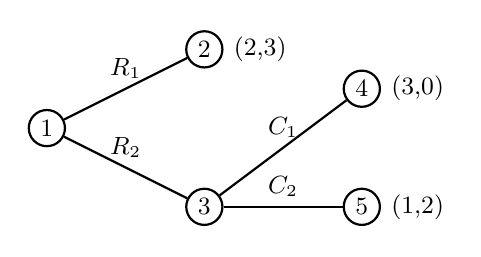
\begin{tikzpicture}[thick,
    p/.style={circle,draw,thick,inner sep=2pt,font=\small},
    out/.style={font=\small},
    opt/.style={above,font=\small},
    every label/.style={font=\small}]
  \node[p] (1) at (0,0) {1};
  \node[p,label=right:{(2,3)}] (2) at (2,1) {2};
  \node[p] (3) at (2,-1) {3};
  \draw (1) -- node[opt] {$R_1$} (2);
  \draw (1) -- node[opt] {$R_2$} (3);
  \node[p,label=right:{(3,0)}] (4) at (4,0.5) {4};
  \node[p,label=right:{(1,2)}] (5) at (4,-1) {5};
  \draw (3) -- node[opt] {$C_1$} (4);
  \draw (3) -- node[opt] {$C_2$} (5);
\end{tikzpicture}
\end{center}

\cmnt{%
  If nodes are connected by dotted lines, then the relevant player
  cannot tell if she is in one of those nodes at which of them she
  is. Such nodes form an \emph{information set}. Games in which there
  can be ignorance about the present node are said to have
  \emph{imperfect information}.%
} %

From a decision theoretic perspective, a game with several moves is a
series of (potential) decision problems, one for each occasion where a
player faces a choice. The states in these decision problems specify
the future decisions of all players. As before, under the assumption
that the utilities and rationality of players are common knowledge, we
can often predict what will happen without specifying the players'
degrees of belief.

Consider the node labelled `3' in the above tree. Here, Column faces a
choice between outcome 4 and outcome 5. That choice involves no
relevant uncertainty, and Column prefers outcome 5. So Column can be
expected to play $C_2$. Anticipating this, Row can figure out that if
she plays $R_2$, then outcome 5 will come about, which has utility 1
for Row. By comparison, if she plays $R_1$, she guarantees outcome 2,
which has utility 2. So Row will play $R_1$.

This process for solving games with multiple moves is called
\textbf{backward induction}. It can lead to very strange results.

\cmnt{%

  A game tree can be reduced to a simple decision matrix by pretending
  that all players decide at the outset on a \emph{strategy} that
  settles what they will choose at each point they might reach, with
  the constraint that the same choice must be made at each point in an
  information set. The resulting matrix is known as the
  \emph{strategic normal form} of the game tree.

  The outcome of an interaction often depends not only on their
  individual choices, but also on external matters, e.g. on whether
  some restaurant is open. Game theory accommodates this by using
  ``lotteries'' as outcomes. For instance, if I want to meet you, and
  we both end up at the restaurant, the outcome might be the complex
  state of affairs $\bet{\emph{Open}}{\emph{Meet \& Eat}}{\emph{Meet
      \& $\neg$Eat}}$. The utility of this state of affairs then
  depends on the probability that the restaurant is open. Since game
  theory tries to avoid specifying subjective probabilities, it is
  usually assumed that the relevant events have an objective chance
  which is common knowledge among all players. Thus it might be
  specified that all parties know that the restaurant owner each day
  decides whether to open her restaurant based on a fair coin toss.

  It's important to treat such games not in normal form. That's
  because the normal form ignores information that can arrive during a
  game. In particular, an agent might play something unexpected and
  this might change what the other agent should do.
} %

\begin{example}[Centipede]
  You and Bob are playing a game. Initially, there's a pot containing
  £2. In round 1, you begin by deciding whether to continue or end the
  game. If you end the game, you get the £2 and Bob gets £0. If you
  continue, the money in the pot increases by £2 and Bob decides
  whether to continue or end. If he ends the game here (in round 2),
  he gets £3 and you get £1. If he continues, the money in the pot
  increases by £2 and it's your turn again. If you end the game 
  (in round 3), you get £4 and Bob gets £2. And so on. In each round,
  the money in the pot increases by £2 and whoever ends the game gets
  £2 more than the other player. In round 100, Bob no longer has an
  option to continue.
\end{example}
Suppose you and Bob don't care about each other; each of you only
wants to get as much money as possible. Here is a partial diagram of the resulting game of Centipede.

\begin{center}
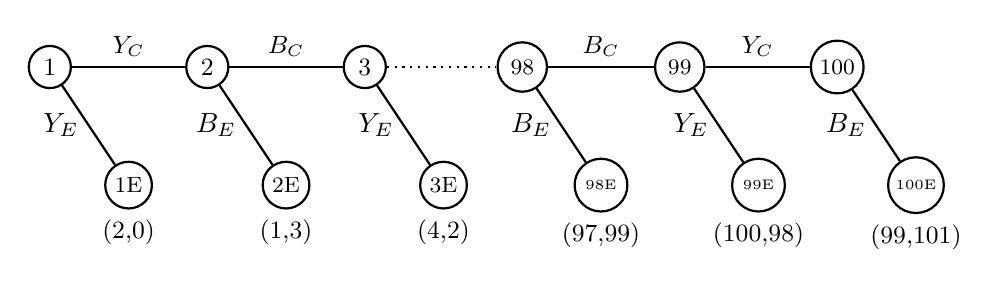
\begin{tikzpicture}[thick,
    p/.style={circle,draw,thick,inner sep=2pt,font=\small},
    xp/.style={circle,draw,thick,inner sep=2pt,font=\footnotesize},
    xxp/.style={circle,draw,thick,inner sep=2pt,font=\tiny},
    out/.style={font=\small},
    opt/.style={above,font=\small},
    every label/.style={font=\small}]
  \node[p] (1) at (0,0) {\,1\,};
  \node[xp,label=below:{(2,0)}] (1E) at (1,-1.5) {1E};
  \draw (1) -- node[left] {$Y_E$} (1E);
  \node[p] (2) at (2,0) {\,2\,};
  \node[xp,label=below:{(1,3)}] (2E) at (3,-1.5) {2E};
  \draw (2) -- node[left] {$B_E$} (2E);
  \draw (1) -- node[opt] {$Y_C$} (2);
  \node[p] (3) at (4,0) {\,3\,};
  \node[xp,label=below:{(4,2)}] (3E) at (5,-1.5) {3E};
  \draw (3) -- node[left] {$Y_E$} (3E);
  \draw (2) -- node[opt] {$B_C$} (3);
  \node[xp] (98) at (6,0) {\,98\,};
  \node[xxp,label=below:{(97,99)}] (98E) at (7,-1.5) {\,98E\,};
  \draw (98) -- node[left] {$B_E$} (98E);
  \draw[dotted] (3) -- (98);
  \node[xp] (99) at (8,0) {\,99\,};
  \node[xxp,label=below:{(100,98)}] (99E) at (9,-1.5) {\,99E\,};
  \draw (99) -- node[left] {$Y_E$} (99E);
  \draw (98) -- node[opt] {$B_C$} (99);
  \node[xp] (100) at (10,0) {100};
  \node[xxp,label=below:{(99,101)}] (100E) at (11,-1.5) {100E};
  \draw (100) -- node[left] {$B_E$} (100E);
  \draw (99) -- node[opt] {$Y_C$} (100);
\end{tikzpicture}
\end{center}

We can use backward induction to figure out how you should play. The
latest point at which a player has a real choice is round 99. Here,
you can either end the game ($Y_E$) and get £100 or continue ($Y_C$)
and get £99. So you should end the game. Anticipating this, what
should Bob do in round 98? If he ends the game ($B_E$), he'll get £99;
if he continues ($B_C$), he'll get £98. So he should end the
game. Anticipating this, you should end the game in round 97, to
ensure that you'll get £98 rather than £97. And so on, all the way
back to round 1. At each point, backward induction tells us the game
should be ended. Thus knowing at round 1 that Bob will end the game in
round 2, you should end the game right away. So the ``solution'' is
that you will get £2 and Bob gets £0.

% \begin{exercise2}
%   Can you think of a real-life situation with a structure similar to
%   the centipede game? 
% \end{exercise2}

When actual people play the Centipede game, almost no-one ends the
game right away. Is this a sign of either altruism or irrationality?
Not necessarily.

Let's look at your choice in round 1 from a decision theoretic
perspective. It is clear what happens if you end the game: you'll get
£2. But what would happen if you decide to continue? The argument from
backward induction assumes that Bob would end the game. And if you
could be certain that Bob would do that, then you should indeed end
the game in round 1. But why should Bob end the game? Because, so the
argument, he can be certain that you would end the game in round 3.
But the argument for ending in round 3 is exactly parallel to the
argument for ending in round 1. Yet if Bob faces a choice in round 2,
then he has just seen that you \emph{didn't} end the game in round 1.
So he arguably can't be sure you would end it in round 3. On the
contrary, he should be somewhat confident that you will continue in
round 3. And then Bob should continue in round 2. It follows that
continuing in round 1 maximizes expected utility, as it is likely to
get you at least to round 3!

\cmnt{%

  is what you would do if I were to play the ``wrong'' move. You would
  learn that either I'm not rational, or you're wrong about the
  utilities, or I believe that you're not rational or that you're
  wrong or that you believe that I'm wrong etc.

} %

\begin{exercise2}
  Change the Centipede game so that there's no fixed end
  point. Rather, each time a player chooses to continue, the game ends
  with a probability of 1\%. Does this change anything? How should
  you play? 
\end{exercise2}

\begin{exercise2}
  Suppose you repeatedly face the Prisoner's Dilemma with the same
  partner, for an unknown number of rounds. You only care about your
  own prison terms. You expect that your partner will remain silent in
  the first round and from then on imitate whatever you did in the
  previous round. In this case, you should arguably remain silent.
  Does that mean you should choose an act that doesn't maximize
  expected utility?
\end{exercise2}


\section{Evolutionary game theory}

\cmnt{%
  Here we are in effect imposing external utilities: we're not
  interesting in the agent's goals, but in what she ought to do in
  order to maximize fitness; in light of information = random or
  correlated pairing.%
} %

One of the most successful applications of game theory lies (somewhat
surprisingly) in the study of biological and cultural
evolution. Consider the following game.

\begin{example}[The Stag Hunt]
  Two players independently decide whether to hunt stag or rabbit.
  Hunting stag requires cooperation, so if only one of the players
  decides to hunt stag, she will get nothing. The utilities are as
  follows.
  \begin{center}
    \begin{tabular}{|r|c|c|}\hline
      \gr & \gr Stag & \gr Rabbit \\\hline
      \gr Stag & 5,5 & 0,1 \\\hline
      \gr Rabbit & 1,0 & 1,1 \\\hline
    \end{tabular}
  \end{center}
\end{example}
\cmnt{%
  Using standard ideas from game theory, we would find the two Nash
  equilibria (Stag,Stag), (Rabbit,Rabbit), which is not much of a
  ``solution''. %
} %

In the evolutionary interpretation, the utilities represent the
\emph{relative fitness} that results from a combination of choices,
measured in terms of average number of surviving offspring. Let's
assume that each strategy is played by a certain fraction of
individuals in a population. Individuals who achieve an outcome with
greater utility will, by definition, have more offspring on average,
so their proportion in the population will increase.

Suppose initially \nicefrac{1}{4} of the individuals in the population
goes for stags and \nicefrac{3}{4} for rabbits. Assuming that
encounters between individuals are completely random, this means that
any given individual has a \nicefrac{1}{4} chance of playing with
someone hunting stag, and a \nicefrac{3}{4} chance of playing with
someone hunting rabbit. The average utility of hunting stag is
therefore $\nicefrac{1}{4} \cdot 5 + \nicefrac{3}{4} \cdot 0 = 1.25$;
for hunting rabbit the utility is of course 1. Individuals going for
stag therefore have greater average fitness. Their fraction in the
population increases. As a consequence, it becomes even more
advantageous to go for stag. Eventually, everyone will hunt stag.

By contrast, suppose initially only \nicefrac{1}{10} of the population
goes for stags. Then hunting stag has an average utility of 0.5, which
is less than the utility of hunting rabbit. So the rabbit hunters will
have more offspring, which makes it even worse to hunt
stags. Eventually, everyone will hunt rabbits.

The two outcomes (Stag,Stag) and (Rabbit,Rabbit) are the two Nash
Equilibria in the Stag Hunt. Evolutionary game theory predicts that
the proportion of stag and rabbit hunters in a population will
approach one of these equilibria. 

\cmnt{%
  Notice that unlike in standard game theory, we made no assumptions
  about common knowledge here. The players don't have to know
  anything, and they can be quite irrational. That's because it's not
  the \emph{players} who decide which strategy is optimal and which
  equilibrium will be reached, but \emph{nature}. Individuals aren't
  actually trying to maximise fitness, but they nevertheless behave as
  if they were, because nature selects for individuals with higher
  fitness.
} %

\cmnt{%

  If you think of all possible fractions of strategies as a phase
  space, the equilibrium (Stag, Stag) has a larger basin of attraction
  than (Rabbit, Rabbit). Sometimes, a Nash equilibrium has a
  point-sized basin of attraction, such as $B,B$ in the following
  game:

  \begin{center}
    \begin{tabular}{|r|c|c|}\hline
      \gr & \gr A & \gr B \\\hline
      \gr B & 5,5 & 0,0 \\\hline
      \gr B & 0,0 & 0,0 \\\hline
    \end{tabular}
  \end{center}

  It is very unlikely that this equilibrium could ever be found -- not
  only because it is unlikely that all players start off playing
  B. Rather, even in this case, mutants or intruders playing A will
  quickly take over. 

} %

Not every Nash Equilibrium is a possible end point of evolution
though. For example, if a population repeatedly plays the game of
Chicken, and the players can't recognize in advance who will swerve
and who will go straight, then the asymmetric equilibria (Swerve, Straight)
and (Straight, Swerve) do not mark possible end points of evolutionary
dynamics. But note that in a community in which almost everyone
swerves, you're better off going straight; similarly, in a community
in which almost everyone goes straight, the best choice is to
swerve. Evolution will therefore lead to the third, mixed strategy
equilibrium, which represents a state in which a certain fraction of
the population swerves and the others go straight.

\cmnt{%
  Hunting stag and hunting rabbit are \textbf{evolutionarily stable}
  in the sense that mutants playing the alternative strategy could not
  take over a population of 100\% stag hunters or 100\% rabbit
  hunters.
} %

\cmnt{%
  for all other strategies $Y$,
  \begin{itemize}
  \item \emph{either} $U(X,X) > U(Y,X)$,
  \item \emph{or} $U(X,X) = U(Y,X)$ and $U(X,Y) > U(Y,Y)$.
  \end{itemize}
  The idea is that either $X$ is \emph{strictly} better against itself
  than every alternative, or, if some mutant alternative $Y$ does
  equally good against $X$, then $X$ does better against $Y$ than $Y$
  itself. 
} %

\cmnt{%
  Considerations of mutants and invaders point at a limitation of our
  original dynamical model, which assumed that the ratios in the next
  generation are entirely determined by the ratios in the parent
  generation and their fitness, without mutation and invasion. There are
  more complex models including these factors.

  Notice that unlike in standard game theory, we made no assumptions
  about common knowledge here. The players don't have to know
  anything, and they can be quite irrational. That's because it's not
  the \emph{players} who decide which strategy is optimal and which
  equilibrium will be reached, but \emph{nature}. Individuals aren't
  actually trying to maximise fitness, but they nevertheless behave as
  if they were, because nature selects for individuals with higher
  fitness.

  What exactly is fitness in evolutionary game theory? It is best
  defined by its role: fitness is something such that the more you
  have it, the more creatures like you will exist in the next
  generation. An obvious candidate is number of offspring, but there
  are situations where this isn't adequate, e.g. when the players are
  ants or more generally when players have a choice that helps other
  players of their type to have more offspring. Biologists sometimes
  speak of ``inclusive fitness'' to take such factors into account.
} %

The assumption that individuals in a population are randomly paired
with one another is obviously unrealistic. In reality, individuals are
more likely to interact with members of their own family, which
increases the chances that they will be paired with individuals of the
same type; they might also actively seek out others who share the
relevant traits. Either way, the resulting \textbf{correlated play}
dramatically changes the situation.

For example, consider a population in which individuals repeatedly
play a Prisoner's Dilemma wherein they can either cooperate with each
other (remain silent, in the original scenario) or defect
(confess). Since defectors always do better than cooperators in any
encounter, it may seem that cooperation can never evolve. However,
cooperators do much better when paired with other cooperators than
defectors when paired with defectors. If the extent of correlation is
sufficiently high, cooperators can therefore take over (although
perhaps not completely). 

In many species, one can find altruistic individuals who sacrifice
their own fitness for the sake of others. Evolutionary game theory
explains how this kind of altruism could have evolved.

\begin{exercise1}
  Why can't we expect cooperative behaviour to take over completely in
  the scenario where cooperation spreads through correlated play?
 \end{exercise1}

\begin{exercise1}
  What are the Nash equilibria in the following game (ignoring
  randomization)? Could all the equilibria come about through an
  evolutionary process? 
  \begin{center}
    \begin{tabular}{|r|c|c|}\hline
      \gr & \gr A & \gr B \\\hline
      \gr A & 5,5 & 1,1 \\\hline
      \gr B & 1,1 & 1,1 \\\hline
    \end{tabular}
  \end{center}
\end{exercise1}

\section{Further reading}

The Stanford Encyclopedia entry on game theory provides a fairly comprehensive overview:

\begin{itemize}
\item Don Ross: \href{https://plato.stanford.edu/entries/game-theory/}{``Game Theory''} (2014)
\end{itemize}

The paradox of backward induction is discussed in
\begin{itemize}
\item Philip Pettit and Robert Sugden: \href{https://www.princeton.edu/~ppettit/papers/BackwardInduction_JournalofPhilosophy_1989.pdf}{``The Backward Induction Paradox''} (1989)
\end{itemize}

For a little more on evolutionary game theory, see

\begin{itemize}
\item Brian Skyrms: ``Game Theory, Rationality and Evolution of the Social Contract'' (2000) 
\end{itemize}

\begin{essay}
  Explain the paradox of backward induction. Why is it a paradox? How
  do you think it could be resolved?
\end{essay}


%%% Local Variables: 
%%% mode: latex
%%% TeX-master: "bdrc.tex"
%%% End: